% Options for packages loaded elsewhere
% Options for packages loaded elsewhere
\PassOptionsToPackage{unicode}{hyperref}
\PassOptionsToPackage{hyphens}{url}
\PassOptionsToPackage{dvipsnames,svgnames,x11names}{xcolor}
%
\documentclass[
  letterpaper,
  DIV=11,
  numbers=noendperiod]{scrartcl}
\usepackage{xcolor}
\usepackage[top=30mm,left=20mm,heightrounded]{geometry}
\usepackage{amsmath,amssymb}
\setcounter{secnumdepth}{-\maxdimen} % remove section numbering
\usepackage{iftex}
\ifPDFTeX
  \usepackage[T1]{fontenc}
  \usepackage[utf8]{inputenc}
  \usepackage{textcomp} % provide euro and other symbols
\else % if luatex or xetex
  \usepackage{unicode-math} % this also loads fontspec
  \defaultfontfeatures{Scale=MatchLowercase}
  \defaultfontfeatures[\rmfamily]{Ligatures=TeX,Scale=1}
\fi
\usepackage{lmodern}
\ifPDFTeX\else
  % xetex/luatex font selection
\fi
% Use upquote if available, for straight quotes in verbatim environments
\IfFileExists{upquote.sty}{\usepackage{upquote}}{}
\IfFileExists{microtype.sty}{% use microtype if available
  \usepackage[]{microtype}
  \UseMicrotypeSet[protrusion]{basicmath} % disable protrusion for tt fonts
}{}
\makeatletter
\@ifundefined{KOMAClassName}{% if non-KOMA class
  \IfFileExists{parskip.sty}{%
    \usepackage{parskip}
  }{% else
    \setlength{\parindent}{0pt}
    \setlength{\parskip}{6pt plus 2pt minus 1pt}}
}{% if KOMA class
  \KOMAoptions{parskip=half}}
\makeatother
% Make \paragraph and \subparagraph free-standing
\makeatletter
\ifx\paragraph\undefined\else
  \let\oldparagraph\paragraph
  \renewcommand{\paragraph}{
    \@ifstar
      \xxxParagraphStar
      \xxxParagraphNoStar
  }
  \newcommand{\xxxParagraphStar}[1]{\oldparagraph*{#1}\mbox{}}
  \newcommand{\xxxParagraphNoStar}[1]{\oldparagraph{#1}\mbox{}}
\fi
\ifx\subparagraph\undefined\else
  \let\oldsubparagraph\subparagraph
  \renewcommand{\subparagraph}{
    \@ifstar
      \xxxSubParagraphStar
      \xxxSubParagraphNoStar
  }
  \newcommand{\xxxSubParagraphStar}[1]{\oldsubparagraph*{#1}\mbox{}}
  \newcommand{\xxxSubParagraphNoStar}[1]{\oldsubparagraph{#1}\mbox{}}
\fi
\makeatother

\usepackage{color}
\usepackage{fancyvrb}
\newcommand{\VerbBar}{|}
\newcommand{\VERB}{\Verb[commandchars=\\\{\}]}
\DefineVerbatimEnvironment{Highlighting}{Verbatim}{commandchars=\\\{\}}
% Add ',fontsize=\small' for more characters per line
\usepackage{framed}
\definecolor{shadecolor}{RGB}{241,243,245}
\newenvironment{Shaded}{\begin{snugshade}}{\end{snugshade}}
\newcommand{\AlertTok}[1]{\textcolor[rgb]{0.68,0.00,0.00}{#1}}
\newcommand{\AnnotationTok}[1]{\textcolor[rgb]{0.37,0.37,0.37}{#1}}
\newcommand{\AttributeTok}[1]{\textcolor[rgb]{0.40,0.45,0.13}{#1}}
\newcommand{\BaseNTok}[1]{\textcolor[rgb]{0.68,0.00,0.00}{#1}}
\newcommand{\BuiltInTok}[1]{\textcolor[rgb]{0.00,0.23,0.31}{#1}}
\newcommand{\CharTok}[1]{\textcolor[rgb]{0.13,0.47,0.30}{#1}}
\newcommand{\CommentTok}[1]{\textcolor[rgb]{0.37,0.37,0.37}{#1}}
\newcommand{\CommentVarTok}[1]{\textcolor[rgb]{0.37,0.37,0.37}{\textit{#1}}}
\newcommand{\ConstantTok}[1]{\textcolor[rgb]{0.56,0.35,0.01}{#1}}
\newcommand{\ControlFlowTok}[1]{\textcolor[rgb]{0.00,0.23,0.31}{\textbf{#1}}}
\newcommand{\DataTypeTok}[1]{\textcolor[rgb]{0.68,0.00,0.00}{#1}}
\newcommand{\DecValTok}[1]{\textcolor[rgb]{0.68,0.00,0.00}{#1}}
\newcommand{\DocumentationTok}[1]{\textcolor[rgb]{0.37,0.37,0.37}{\textit{#1}}}
\newcommand{\ErrorTok}[1]{\textcolor[rgb]{0.68,0.00,0.00}{#1}}
\newcommand{\ExtensionTok}[1]{\textcolor[rgb]{0.00,0.23,0.31}{#1}}
\newcommand{\FloatTok}[1]{\textcolor[rgb]{0.68,0.00,0.00}{#1}}
\newcommand{\FunctionTok}[1]{\textcolor[rgb]{0.28,0.35,0.67}{#1}}
\newcommand{\ImportTok}[1]{\textcolor[rgb]{0.00,0.46,0.62}{#1}}
\newcommand{\InformationTok}[1]{\textcolor[rgb]{0.37,0.37,0.37}{#1}}
\newcommand{\KeywordTok}[1]{\textcolor[rgb]{0.00,0.23,0.31}{\textbf{#1}}}
\newcommand{\NormalTok}[1]{\textcolor[rgb]{0.00,0.23,0.31}{#1}}
\newcommand{\OperatorTok}[1]{\textcolor[rgb]{0.37,0.37,0.37}{#1}}
\newcommand{\OtherTok}[1]{\textcolor[rgb]{0.00,0.23,0.31}{#1}}
\newcommand{\PreprocessorTok}[1]{\textcolor[rgb]{0.68,0.00,0.00}{#1}}
\newcommand{\RegionMarkerTok}[1]{\textcolor[rgb]{0.00,0.23,0.31}{#1}}
\newcommand{\SpecialCharTok}[1]{\textcolor[rgb]{0.37,0.37,0.37}{#1}}
\newcommand{\SpecialStringTok}[1]{\textcolor[rgb]{0.13,0.47,0.30}{#1}}
\newcommand{\StringTok}[1]{\textcolor[rgb]{0.13,0.47,0.30}{#1}}
\newcommand{\VariableTok}[1]{\textcolor[rgb]{0.07,0.07,0.07}{#1}}
\newcommand{\VerbatimStringTok}[1]{\textcolor[rgb]{0.13,0.47,0.30}{#1}}
\newcommand{\WarningTok}[1]{\textcolor[rgb]{0.37,0.37,0.37}{\textit{#1}}}

\usepackage{longtable,booktabs,array}
\usepackage{calc} % for calculating minipage widths
% Correct order of tables after \paragraph or \subparagraph
\usepackage{etoolbox}
\makeatletter
\patchcmd\longtable{\par}{\if@noskipsec\mbox{}\fi\par}{}{}
\makeatother
% Allow footnotes in longtable head/foot
\IfFileExists{footnotehyper.sty}{\usepackage{footnotehyper}}{\usepackage{footnote}}
\makesavenoteenv{longtable}
\usepackage{graphicx}
\makeatletter
\newsavebox\pandoc@box
\newcommand*\pandocbounded[1]{% scales image to fit in text height/width
  \sbox\pandoc@box{#1}%
  \Gscale@div\@tempa{\textheight}{\dimexpr\ht\pandoc@box+\dp\pandoc@box\relax}%
  \Gscale@div\@tempb{\linewidth}{\wd\pandoc@box}%
  \ifdim\@tempb\p@<\@tempa\p@\let\@tempa\@tempb\fi% select the smaller of both
  \ifdim\@tempa\p@<\p@\scalebox{\@tempa}{\usebox\pandoc@box}%
  \else\usebox{\pandoc@box}%
  \fi%
}
% Set default figure placement to htbp
\def\fps@figure{htbp}
\makeatother





\setlength{\emergencystretch}{3em} % prevent overfull lines

\providecommand{\tightlist}{%
  \setlength{\itemsep}{0pt}\setlength{\parskip}{0pt}}



 


\KOMAoption{captions}{tableheading}
\makeatletter
\@ifpackageloaded{caption}{}{\usepackage{caption}}
\AtBeginDocument{%
\ifdefined\contentsname
  \renewcommand*\contentsname{Table of contents}
\else
  \newcommand\contentsname{Table of contents}
\fi
\ifdefined\listfigurename
  \renewcommand*\listfigurename{List of Figures}
\else
  \newcommand\listfigurename{List of Figures}
\fi
\ifdefined\listtablename
  \renewcommand*\listtablename{List of Tables}
\else
  \newcommand\listtablename{List of Tables}
\fi
\ifdefined\figurename
  \renewcommand*\figurename{Figure}
\else
  \newcommand\figurename{Figure}
\fi
\ifdefined\tablename
  \renewcommand*\tablename{Table}
\else
  \newcommand\tablename{Table}
\fi
}
\@ifpackageloaded{float}{}{\usepackage{float}}
\floatstyle{ruled}
\@ifundefined{c@chapter}{\newfloat{codelisting}{h}{lop}}{\newfloat{codelisting}{h}{lop}[chapter]}
\floatname{codelisting}{Listing}
\newcommand*\listoflistings{\listof{codelisting}{List of Listings}}
\makeatother
\makeatletter
\makeatother
\makeatletter
\@ifpackageloaded{caption}{}{\usepackage{caption}}
\@ifpackageloaded{subcaption}{}{\usepackage{subcaption}}
\makeatother
\usepackage{bookmark}
\IfFileExists{xurl.sty}{\usepackage{xurl}}{} % add URL line breaks if available
\urlstyle{same}
\hypersetup{
  pdftitle={CHL5233: EDA in-class assignment},
  pdfauthor={Qiulei Xu},
  colorlinks=true,
  linkcolor={blue},
  filecolor={Maroon},
  citecolor={Blue},
  urlcolor={Blue},
  pdfcreator={LaTeX via pandoc}}


\title{CHL5233: EDA in-class assignment}
\author{Qiulei Xu}
\date{}
\begin{document}
\maketitle


\begin{Shaded}
\begin{Highlighting}[]
\FunctionTok{library}\NormalTok{(dplyr)}
\end{Highlighting}
\end{Shaded}

\begin{verbatim}

Attaching package: 'dplyr'
\end{verbatim}

\begin{verbatim}
The following objects are masked from 'package:stats':

    filter, lag
\end{verbatim}

\begin{verbatim}
The following objects are masked from 'package:base':

    intersect, setdiff, setequal, union
\end{verbatim}

\begin{Shaded}
\begin{Highlighting}[]
\FunctionTok{library}\NormalTok{(ggplot2)}
\FunctionTok{library}\NormalTok{(readr)}

\CommentTok{\# Load the prepared dataset}
\NormalTok{data }\OtherTok{\textless{}{-}} \FunctionTok{read\_csv}\NormalTok{(}\StringTok{"../data/processed/final\_data.csv"}\NormalTok{)}
\end{Highlighting}
\end{Shaded}

\begin{verbatim}
Rows: 3720 Columns: 17
\end{verbatim}

\begin{verbatim}
-- Column specification --------------------------------------------------------
Delimiter: ","
chr  (1): iso
dbl (16): year, maternal_mortality, infant_mortality, neonatal_mortality, un...

i Use `spec()` to retrieve the full column specification for this data.
i Specify the column types or set `show_col_types = FALSE` to quiet this message.
\end{verbatim}

\begin{Shaded}
\begin{Highlighting}[]
\CommentTok{\# Check data structure}
\FunctionTok{glimpse}\NormalTok{(data)}
\end{Highlighting}
\end{Shaded}

\begin{verbatim}
Rows: 3,720
Columns: 17
$ iso                <chr> "AFG", "AFG", "AFG", "AFG", "AFG", "AFG", "AFG", "A~
$ year               <dbl> 2000, 2001, 2002, 2003, 2004, 2005, 2006, 2007, 200~
$ maternal_mortality <dbl> 1450, 1390, 1300, 1240, 1180, 1140, 1120, 1090, 103~
$ infant_mortality   <dbl> 90.5, 87.9, 85.3, 82.7, 80.0, 77.3, 74.6, 71.9, 69.~
$ neonatal_mortality <dbl> 60.9, 59.7, 58.5, 57.2, 55.9, 54.6, 53.2, 51.7, 50.~
$ under5_mortality   <dbl> 129.2, 125.2, 121.1, 116.9, 112.6, 108.4, 104.1, 99~
$ earthquake         <dbl> 0, 1, 1, 1, 1, 1, 1, 0, 0, 1, 1, 0, 1, 1, 0, 1, 0, ~
$ drought            <dbl> 1, 0, 0, 0, 0, 0, 1, 0, 1, 0, 0, 1, 0, 0, 0, 0, 0, ~
$ armed_conflict     <dbl> 1, 1, 1, 1, 1, 1, 1, 1, 1, 1, 1, 1, 1, 1, 1, 1, 1, ~
$ gdp_1000           <dbl> NA, NA, 0.1835328, 0.2004626, 0.2216576, 0.2550551,~
$ oecd               <dbl> 0, 0, 0, 0, 0, 0, 0, 0, 0, 0, 0, 0, 0, 0, 0, 0, 0, ~
$ pop_dens           <dbl> 14.136539, 14.231558, 14.322705, 14.406906, 15.2194~
$ urban              <dbl> 16.25324, 16.25661, 16.42654, 16.60701, 16.71367, 1~
$ age_dep            <dbl> 108.34663, 108.98989, 109.34716, 109.44753, 109.286~
$ male_edu           <dbl> 2.762086, 2.856936, 2.954241, 3.054121, 3.156706, 3~
$ temp               <dbl> 12.69959, 12.85570, 12.71081, 12.16592, 13.04643, 1~
$ rainfall_1000      <dbl> 0.2763704, 0.2793079, 0.3805710, 0.4288939, 0.37543~
\end{verbatim}

\begin{Shaded}
\begin{Highlighting}[]
\CommentTok{\# Check missing values}
\FunctionTok{colSums}\NormalTok{(}\FunctionTok{is.na}\NormalTok{(data))}
\end{Highlighting}
\end{Shaded}

\begin{verbatim}
               iso               year maternal_mortality   infant_mortality 
                 0                  0                426                 20 
neonatal_mortality   under5_mortality         earthquake            drought 
                20                 20                  0                  0 
    armed_conflict           gdp_1000               oecd           pop_dens 
                 0                 62                  0                 20 
             urban            age_dep           male_edu               temp 
                20                  0                 20                 20 
     rainfall_1000 
                20 
\end{verbatim}

\begin{Shaded}
\begin{Highlighting}[]
\CommentTok{\# Count affected countries by year}
\NormalTok{conflict\_by\_year }\OtherTok{\textless{}{-}}\NormalTok{ data }\SpecialCharTok{|\textgreater{}}
  \FunctionTok{group\_by}\NormalTok{(year) }\SpecialCharTok{|\textgreater{}}
  \FunctionTok{summarise}\NormalTok{(}
    \AttributeTok{affected\_countries =} \FunctionTok{sum}\NormalTok{(armed\_conflict }\SpecialCharTok{==} \DecValTok{1}\NormalTok{),}
    \AttributeTok{.groups =} \StringTok{"drop"}
\NormalTok{  )}

\FunctionTok{print}\NormalTok{(conflict\_by\_year)}
\end{Highlighting}
\end{Shaded}

\begin{verbatim}
# A tibble: 20 x 2
    year affected_countries
   <dbl>              <int>
 1  2000                 39
 2  2001                 40
 3  2002                 40
 4  2003                 32
 5  2004                 34
 6  2005                 36
 7  2006                 37
 8  2007                 29
 9  2008                 31
10  2009                 37
11  2010                 32
12  2011                 28
13  2012                 32
14  2013                 29
15  2014                 31
16  2015                 32
17  2016                 38
18  2017                 49
19  2018                 39
20  2019                 39
\end{verbatim}

\begin{Shaded}
\begin{Highlighting}[]
\CommentTok{\#Code for the time{-}trend analysis}
\FunctionTok{ggplot}\NormalTok{(conflict\_by\_year,}
       \FunctionTok{aes}\NormalTok{(}\AttributeTok{x =}\NormalTok{ year, }\AttributeTok{y =}\NormalTok{ affected\_countries)) }\SpecialCharTok{+}
  \FunctionTok{geom\_line}\NormalTok{(}\AttributeTok{color =} \StringTok{"steelblue"}\NormalTok{, }\AttributeTok{linewidth =} \DecValTok{1}\NormalTok{) }\SpecialCharTok{+}
  \FunctionTok{geom\_point}\NormalTok{(}\AttributeTok{color =} \StringTok{"steelblue"}\NormalTok{, }\AttributeTok{size =} \DecValTok{2}\NormalTok{) }\SpecialCharTok{+}
  \FunctionTok{scale\_x\_continuous}\NormalTok{(}\AttributeTok{breaks =} \FunctionTok{seq}\NormalTok{(}\DecValTok{2000}\NormalTok{, }\DecValTok{2019}\NormalTok{, }\DecValTok{2}\NormalTok{)) }\SpecialCharTok{+}
  \FunctionTok{labs}\NormalTok{(}
    \AttributeTok{title =} \StringTok{"Countries Experiencing Armed Conflict"}\NormalTok{,}
    \AttributeTok{subtitle =} \StringTok{"2000–2019"}\NormalTok{,}
    \AttributeTok{x =} \StringTok{"Year"}\NormalTok{,}
    \AttributeTok{y =} \StringTok{"Number of Countries"}
\NormalTok{  ) }\SpecialCharTok{+}
  \FunctionTok{theme\_minimal}\NormalTok{()}
\end{Highlighting}
\end{Shaded}

\pandocbounded{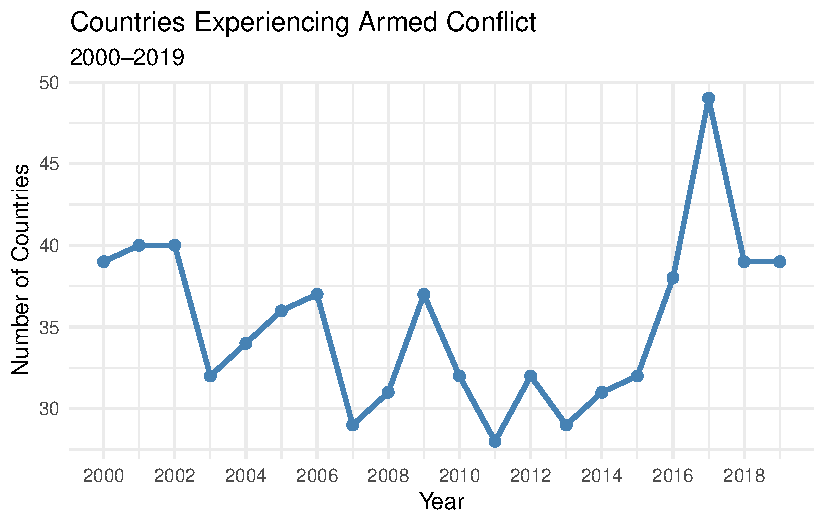
\includegraphics[keepaspectratio]{Class_5_EDA_files/figure-pdf/unnamed-chunk-2-1.pdf}}

\begin{Shaded}
\begin{Highlighting}[]
\CommentTok{\# Highest number of affected countries}
\NormalTok{conflict\_by\_year }\SpecialCharTok{|\textgreater{}}
  \FunctionTok{slice\_max}\NormalTok{(affected\_countries, }\AttributeTok{n =} \DecValTok{1}\NormalTok{)}
\end{Highlighting}
\end{Shaded}

\begin{verbatim}
# A tibble: 1 x 2
   year affected_countries
  <dbl>              <int>
1  2017                 49
\end{verbatim}

\begin{Shaded}
\begin{Highlighting}[]
\CommentTok{\# Lowest number of affected countries}
\NormalTok{conflict\_by\_year }\SpecialCharTok{|\textgreater{}}
  \FunctionTok{slice\_min}\NormalTok{(affected\_countries, }\AttributeTok{n =} \DecValTok{1}\NormalTok{)}
\end{Highlighting}
\end{Shaded}

\begin{verbatim}
# A tibble: 1 x 2
   year affected_countries
  <dbl>              <int>
1  2011                 28
\end{verbatim}

\subsubsection{Exploratory Data Analysis: Armed
Conflict}\label{exploratory-data-analysis-armed-conflict}

I explored how the number of countries experiencing armed conflict
changed from 2000 to 2019. The dataset contains observations from 186
countries over 20 years. I first checked for missing values and found
that the armed conflict indicator had no missing observations. Then, I
grouped the data by year and calculated the number of countries
experiencing armed conflict each year. I used a line plot to visualize
the changes over time.

The results showed that the number of affected countries fluctuated
throughout the study period. The highest number was recorded in 2017,
with 49 countries, while the lowest was in 2011, with 28 countries.
There was a noticeable increase between 2015 and 2017, followed by a
decrease in 2018. Overall, the results do not suggest a consistent
increasing or decreasing trend over the entire period.

\begin{Shaded}
\begin{Highlighting}[]
\CommentTok{\#Exploring the relationship between armed conflict and under{-}five mortality}
\NormalTok{mortality\_data }\OtherTok{\textless{}{-}}\NormalTok{ data }\SpecialCharTok{|\textgreater{}}
  \FunctionTok{filter}\NormalTok{(}\SpecialCharTok{!}\FunctionTok{is.na}\NormalTok{(under5\_mortality)) }\SpecialCharTok{|\textgreater{}}
  \FunctionTok{mutate}\NormalTok{(}
    \AttributeTok{conflict\_status =} \FunctionTok{factor}\NormalTok{(}
\NormalTok{      armed\_conflict,}
      \AttributeTok{levels =} \FunctionTok{c}\NormalTok{(}\DecValTok{0}\NormalTok{, }\DecValTok{1}\NormalTok{),}
      \AttributeTok{labels =} \FunctionTok{c}\NormalTok{(}\StringTok{"No Conflict"}\NormalTok{, }\StringTok{"Conflict"}\NormalTok{)}
\NormalTok{    )}
\NormalTok{  )}

\FunctionTok{ggplot}\NormalTok{(mortality\_data,}
       \FunctionTok{aes}\NormalTok{(}\AttributeTok{x =}\NormalTok{ conflict\_status, }\AttributeTok{y =}\NormalTok{ under5\_mortality,}
           \AttributeTok{fill =}\NormalTok{ conflict\_status)) }\SpecialCharTok{+}
  \FunctionTok{geom\_boxplot}\NormalTok{(}\AttributeTok{alpha =} \FloatTok{0.7}\NormalTok{) }\SpecialCharTok{+}
  \FunctionTok{labs}\NormalTok{(}
    \AttributeTok{title =} \StringTok{"Under{-}Five Mortality by Armed Conflict Status"}\NormalTok{,}
    \AttributeTok{subtitle =} \StringTok{"2000–2019"}\NormalTok{,}
    \AttributeTok{x =} \StringTok{"Armed Conflict Status"}\NormalTok{,}
    \AttributeTok{y =} \StringTok{"Under{-}Five Mortality (per 1,000 live births)"}
\NormalTok{  ) }\SpecialCharTok{+}
  \FunctionTok{theme\_minimal}\NormalTok{() }\SpecialCharTok{+}
  \FunctionTok{theme}\NormalTok{(}\AttributeTok{legend.position =} \StringTok{"none"}\NormalTok{)}
\end{Highlighting}
\end{Shaded}

\pandocbounded{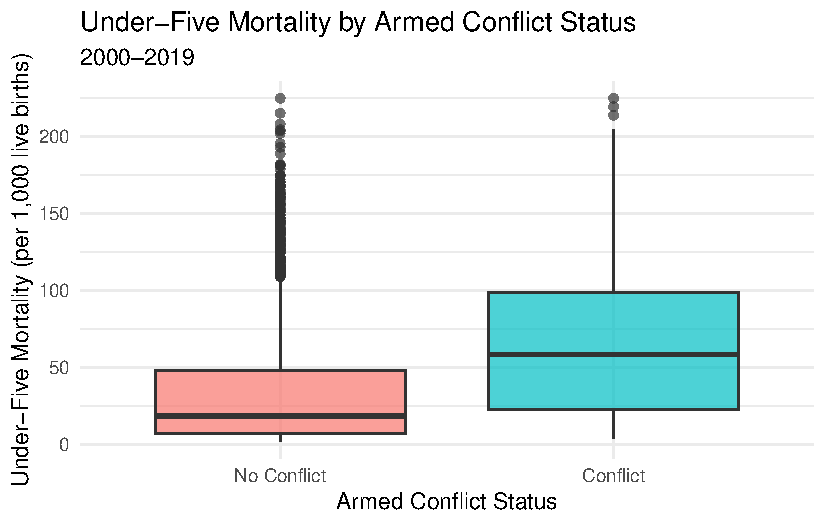
\includegraphics[keepaspectratio]{Class_5_EDA_files/figure-pdf/unnamed-chunk-3-1.pdf}}

\begin{Shaded}
\begin{Highlighting}[]
\NormalTok{mortality\_by\_year }\OtherTok{\textless{}{-}}\NormalTok{ mortality\_data }\SpecialCharTok{|\textgreater{}}
  \FunctionTok{group\_by}\NormalTok{(year, conflict\_status) }\SpecialCharTok{|\textgreater{}}
  \FunctionTok{summarise}\NormalTok{(}
    \AttributeTok{mean\_mortality =} \FunctionTok{mean}\NormalTok{(under5\_mortality),}
    \AttributeTok{.groups =} \StringTok{"drop"}
\NormalTok{  )}

\FunctionTok{ggplot}\NormalTok{(mortality\_by\_year,}
       \FunctionTok{aes}\NormalTok{(}\AttributeTok{x =}\NormalTok{ year,}
           \AttributeTok{y =}\NormalTok{ mean\_mortality,}
           \AttributeTok{color =}\NormalTok{ conflict\_status)) }\SpecialCharTok{+}
  \FunctionTok{geom\_line}\NormalTok{(}\AttributeTok{linewidth =} \DecValTok{1}\NormalTok{) }\SpecialCharTok{+}
  \FunctionTok{geom\_point}\NormalTok{(}\AttributeTok{size =} \FloatTok{1.5}\NormalTok{) }\SpecialCharTok{+}
  \FunctionTok{labs}\NormalTok{(}
    \AttributeTok{title =} \StringTok{"Under{-}Five Mortality by Conflict Status"}\NormalTok{,}
    \AttributeTok{subtitle =} \StringTok{"2000–2019"}\NormalTok{,}
    \AttributeTok{x =} \StringTok{"Year"}\NormalTok{,}
    \AttributeTok{y =} \StringTok{"Mean Under{-}Five Mortality (per 1,000)"}\NormalTok{,}
    \AttributeTok{color =} \StringTok{"Conflict Status"}
\NormalTok{  ) }\SpecialCharTok{+}
  \FunctionTok{theme\_minimal}\NormalTok{()}
\end{Highlighting}
\end{Shaded}

\pandocbounded{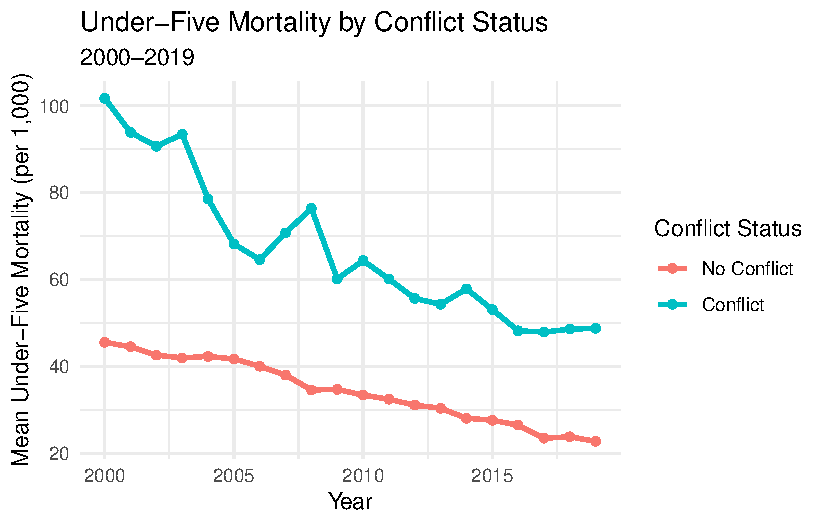
\includegraphics[keepaspectratio]{Class_5_EDA_files/figure-pdf/unnamed-chunk-3-2.pdf}}

\paragraph{Exploring the Relationship Between Armed Conflict and
Under-Five
Mortality}\label{exploring-the-relationship-between-armed-conflict-and-under-five-mortality}

As an extension of the time-trend analysis, I explored the relationship
between armed conflict and under-five mortality from 2000 to 2019. I
grouped the observations by armed conflict status and calculated
descriptive statistics for under-five mortality. The mean mortality rate
was approximately 66.86 per 1,000 live births for country-years
experiencing armed conflict, compared with 34.31 for those without
conflict. I used a boxplot to compare the distributions and a line plot
to examine how mortality rates changed over time.

The results showed that under-five mortality was consistently higher in
the conflict group throughout the study period. Both groups experienced
declining mortality rates over time, but the difference between them
remained substantial. These findings suggest an association between
armed conflict and higher under-five mortality. However, further
analysis would be necessary to account for other factors that may
influence mortality rates.




\end{document}
